\section{Architecture of \sys{}}

A key contribution of this work is the design and implementation of the \sys artifact, which provides a practical, performant, and extensible system for studying overlay multicast algorithms in cloud environments.
The \sys{} system simplifies the design and deployment of multicast overlays spanning cloud object stores.
%\sys{} is highly extensible and supports pluggable algorithms for determining the location and number of overlay nodes to be created as well as the paths along with data is replicated.  
We use it to implement and deploy the optimizer described in \cref{sec:optimization} and several baseline algorithms.



%\sarah{is it necessary to discuss the differences/extensions needed to be made to Skyplane?}




\begin{figure}[t]
    \centering
    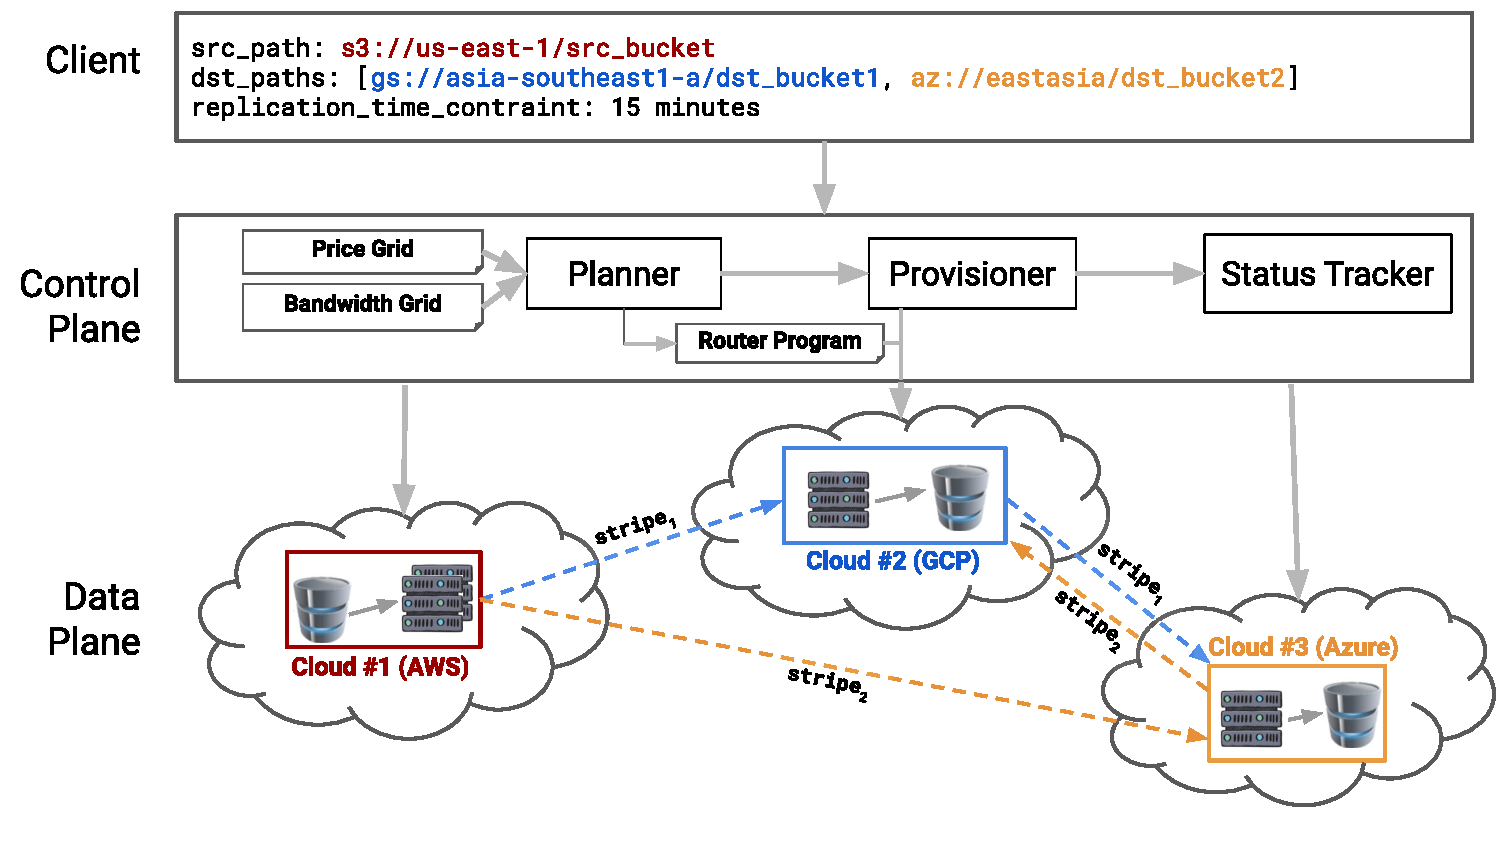
\includegraphics[width=\linewidth]{figures/cloudcast-architecture.pdf}
    % https://docs.google.com/presentation/d/1o04fk0svMe0Rg8bzGh-totPuRxAksQeNfPcIyaaWJgY/edit#slide=id.p
    \caption{\sys{} system architecture.}
    \label{fig:architecture}
\end{figure}




%To implement optimized multicast replication trees as well as baseline algorithms for real cloud replications, we develop \sys{}, a system for bulk data multicast between cloud object stores or VMs. \sys{} uses a user-provided target replication time and data path to determine a \textit{multicast plan} with the optimizer described in \cref{sec:optimization}, which identifies the location and number of overlay nodes to be created as well as how data should be replicated across the overlay. \sys{} then deploys cloud VMs to construct the overlay network and execute the replication as specified by the multicast plan. 


We provide an overview of \sys{} in \cref{fig:architecture}. \sys{} is designed with a centralized control plane and a distributed data plane. The control plane determines the set of overlay nodes and routing paths, and it dispatches and monitors multicast jobs. The data plane consists of \textit{overlay routers}, which we implement as modular software routers running on overlay nodes deployed on cloud VMs. \sarah{is this correct?} The control plane configures overlay routers using a \textit{router program}, which specifies a graph of modular operators for processing data.
Each overlay router gets a unique router program, which, in cooperation with other routers in the system, implements the desired flow of data over the overlay network.

\sys is implemented as part of the Skyplane \cite{jain2022skyplane} open source project and consisted of \todo{$\sim$18K} additional lines of Python to implement the \todo{overlay routers and XXX}.


\subsection{Control Plane}
%\sys{} uses a centralized control plane that can run on the client's machine or as a service in the cloud, and is responsible for initiating and monitoring replication.  
The control plane contains the planner, which supports pluggable algorithms for determining the placement of overlay routers across cloud providers and paths along which data is replicated (shown in \cref{fig:architecture}).
The output of the planner is used to provision VMs to act as overlay routers across cloud regions and to compile a router program for each overlay router that configures its behavior.
Finally, the control plane initiates the transfer and monitors its progress. 

\heading{Planner} 
The planner is responsible for creating a multicast plan based on a target replication time, source and destination object store paths provided by the user, and profiling data described in \cref{ss:profiling}.  
The planner takes as input the algorithm to use for generating a multicast plan, which can be the default \sys{} optimizer described in \cref{sec-optimizer} or a custom plan (e.g., a Steiner Tree over the cost graph). The planning algorithm determines how many overlay nodes to create in each region and how each data stripe should be routed through the overlay network. The planner uses the algorithm output to generate a \textit{router program} for each overlay router, which specifies how the overlay router should process a chunk header when received. 
The \sys{} default optimizer is implemented using Python's CVXPY library \cite{cvxpy} (version 1.3.2) with a Gurobi solver \cite{gurobi}, implemented in about $1$K lines of code.  

\heading{Provisioner} 
Once a multicast plan is determined, the provisioner instantiates the overlay routers.
The provisioner creates a VPC in each cloud provider and provisions VMs to act as overlay routers within these VPCs.
The provisioner also sets firewall rules to allow network traffic between overlay routers, which send and receive data from each other, as specified by the planner-generated router programs. 
Once a VM has been instantiated, the provisioner
installs and launches the router programs as containers on the VMs.

\heading{Chunk Dispatching and Status Tracker} 
The control plane subdivides replication target data into \textit{chunks}, which are at most 64MB in size, to allow for transfer pipelining and parallelism.
%Chunks are similar to packets but are larger to reduce metadata overhead.
Each chunk has a \textit{chunk header}, which specifies a key (e.g., object store object, filename), byte range, and an optional multipart ID (required for multipart uploads).
The chunk header also contains a \textit{stripe ID}, which specifies which path along the overlay the chunk will take. 

The control plane informs each source overlay router (i.e., overlay routers responsible for reading source data) the chunks for which they are responsible by sending the corresponding chunk headers.
We refer to this as \textit{registering} a chunk to an overlay router. 
%The control plane also uses cloud APIs to initiate multipart upload requests for large objects which are divided into multiple chunks. 
The control plane's status tracker monitors the status of each chunk by querying the status of chunks on each overlay router. 
%The controller maintains a status bar for transfer progress by monitoring chunk IDs marked as completed on the destination overlay routers (responsible for writing to the destination object store). 
%After all chunks have been completed processing, the controller finalizes the transfer by calling cloud provider APIs to mark any multipart upload requests are completed, and deprovisions the overlay routers. 
%These operations that directly interface with cloud API are separate from data plane operations.
% The status tracker also performs necessary logging and monitoring actions to ensure the transfer process is visible to end users. 

%\begin{comment}
%    \begin{lstlisting}[float=tp,basicstyle=\ttfamily\footnotesize,language=Python,caption={Example API call using the \sys{} solver.}, label={lst:api-example}]
%client = CloudcastClient()
%tracker = client.copy_async(
%    src="s3://source_bucket", 
%    dests=["s3://dest_bucket1", "gcp://dest_bucket2", "azure://dest_bucket3"], 
%    recursive=True, 
%    algorithm="cloudcast_opt",
%    replication_time_constraint_s=300
%)
%# monitor transfer status
%remaining_bytes = tracker.query_bytes_remaining()
%\end{lstlisting}
%\end{comment}


\subsection{Data Plane}
The data plane is composed of overlay routers, each running on a single VM. 
The overlay routers are created and configured by the control plane to execute the transfer according to the multicast plan. 
\sys{} supports configurable overlays by defining processing on overlay routers using modular operators, inspired by the design of configurable routers \cite{kohler2000click}.

The router program provided by the control plane specifies a directed acyclic graph (DAG) of \textit{operators} (analogous to elements) and \textit{connections}, all of which run on each overlay router and are used to process incoming chunk headers registered to the overlay router. \sarah{Should we just call them queues and operators, rather than using the click terminology?}
The DAGs are created at the overlay router's startup time based on the router program, and they allow overlay routers to process chunks without additional coordination with the control plane.

%elements are individual chunk processing modules, such as reading the chunk from the source object store, relaying the chunk to another overlay router's IP, or writing the chunk to a destination object store. Connections are queues that pass chunk headers between elements, and can be configured to send a chunk header to one or all of multiple downstream elements. 
%Each stripe ID corresponds to a unique DAG (so that different stripes can be routed differently). Chunk processing is pre-configured on each overlay router by the router program, and does not require any additional coordination with the control plane to decide how to process chunks.
%
%Each overlay router runs an HTTP server which receives chunk registrations (containing chunk header information), which the overlay router then processes via a DAG of \textit{elements} and \textit{connections}. 

\begin{table*}[t!]
\centering
\footnotesize
\renewcommand{\arraystretch}{1.1}
\begin{tabularx}{\textwidth}{ l X }
\toprule
    \textbf{System} & \textbf{Description} \\
    \midrule
    Direct & Data is transferred directly from the source to the destination regions.  \\
    MDST & Data is transferred along edges selected by a Minimum Directed Spanning Tree (including source and destination regions) computed from network costs. \\
    Steiner Tree & Data is transferred along edges selected by a Steiner tree (including optional waypoint regions) computed from network costs. \\
    SPIDER~\cite{ganguly2005fast} & Data is transferred according to the plan generated by SPIDER, a system designed for fast bulk replication to multiple destinations.\\
    Skyplane & Skyplane's optimizer is used to select paths for each source-destination pair, which are combined to build the distribution tree.  \\
    CloudMPCast~\cite{garcia2015cost} & Data is transferred over a set of cost-minimizing edges that meet a minimum bandwidth threshold. \\
    %\makecell[tl]{Cost-aware\\ Inter-DC Multicast~\cite{fatemipour2022cost}} & Data is transferred according to a solver that models cost and deadlines in the inter-DC context (e.g., bandwidth and switch-based pricing) according to \cite{fatemipour2022cost}. \\
    \makecell[tl]{Deadline-aware\\ Inter-DC Multicast~\cite{deadline2018}} & Data is transferred to meet deadlines in the inter-DC context according to \cite{deadline2018}. Note that due to scalability issues, we needed to modify the candidate tree generation step to only consider a subset of waypoint regions to achieve tractable runtimes. \\
    \makecell[tl]{AWS S3 Multi-\\Region Bucket~\cite{aws-replication}} & Vendor product that supports intra-cloud between AWS regions only. We enable Replication Time Control~\cite{aws-replication-time-control}.\\
    Bullet~\cite{kostic2003bullet} &  Data is transferred according to the plan generated by Bullet, a high-bandwidth dissemination technique using an overlay mesh.\\
    BitTorrent~\cite{twitter-bittorrent} & Peer-to-peer protocol where peers download data from each other in a decentralized manner.\\
    \midrule
    Cloudcast-Opt (HT) & Data is transferred along the highest throughput (HT) multicast tree generated by our optimizer (tightest time constraint).\\
    Cloudcast-Opt (LC) & Data is transferred along a low cost (LC) multicast tree generated by our optimizer (relatively loose time constraint).\\
    \bottomrule
\end{tabularx}
\caption{All of the systems and variants we evaluate, covering a mix of academic baselines and commercial solutions.}
\label{tab:baselines}
\end{table*}

Operators are implemented as a pool of worker processes running processing steps for a chunk, such as reading the chunk from the source object store, relaying the chunk to another overlay router, writing the chunk to a destination object store, or transforming the chunk data (e.g., compression or encryption).  Connections pass chunk headers between operators via thread-safe queues, and can be configured to send a chunk header to one or all of multiple downstream operators. 
%Although not used in our evaluation, by default, the object store download element is followed by elements to compress (via LZ4) and encrypt (\textcolor{red}{(todo:cite)})  chunk data; similarly, the object store upload is preceded by decompression and decryption. 
%New transformations to chunks (e.g. a different compression function) can be added by modifying the router program in the control plane. 
%The first element in the DAG must retrieve the data corresponding to some chunk header, either by downloading from the source object store or recieving data from another overlay router. 

For example, on a source overlay router, chunk registrations from the control plane will provide chunk headers to the first operator in the DAG, which downloads chunk data from an object store. All chunk data is stored in a shared memory filesystem to allow for fast access across operators. Once chunk data is downloaded, the chunk header is passed to the next operator via a connection, which runs LZ4 compression \cite{lz4}) and secret key encryption \cite{pynacl, libsodium} on the chunk data. The leaf operators are `sender' operators, which relay the chunk header and data to other overlay routers. 

%\heading{Relaying Chunk Between Overlay Routers} 
Chunk data is relayed between overlay routers by a `sender' operator on the sending router and a `receiver' operator on the receiving overlay router.
When the sender operator is created, it creates parallel TCP connections 
%(specified by the router program of the receiving overlay router), 
which are kept open for the duration of the transfer. 
Before sending chunk data, the sender will attempt to register the corresponding chunk headers with the receiving overlay router to ensure it has space in its shared memory file system to write the chunk data. Once chunks are registered, the sender will send the chunk data over the TCP sockets, and the receiver will wait for the written chunk data size to match the size specified by the chunk header, before sending chunk headers to the next operator. Successfully sent chunk data is deleted from the shared memory filesystem. 

\heading{Backpressure}  Connections are configured with a maximum size for the underlying queues. If the queue reaches its maximum size, the upstream operator will wait until the queue size decreases sending chunk headers to the connection.

\heading{Striping} Registered chunk headers with different stripe IDs are placed in different queues and processed by separate DAGs, so that different stripes can be routed differently.




%\subsection{Usage}

%\sys{} users can run multicast replication jobs using either a Python API or a CLI command.
%\sys{} requires that users authenticate with cloud provider CLI tools, which enable cached credentials to provision resources on the user's behalf to execute transfer requests.
%Listing~\ref{lst:api-example} shows an example of how a user specifies the source/destination paths and replication time constraints using the Python client. 
